\begin{frame}
  \frametitle{JDK的下载和安装}
  \begin{enumerate}
    \item 利用搜索引擎,找到Oracle JDK的官方下载页面:\href{http://www.oracle.com/technetwork/cn/java/javase/downloads/index.html}{Java SE 下载}
    \item 根据自己操作系统的类型,选择下载对应版本的Java SE 8 JDK
      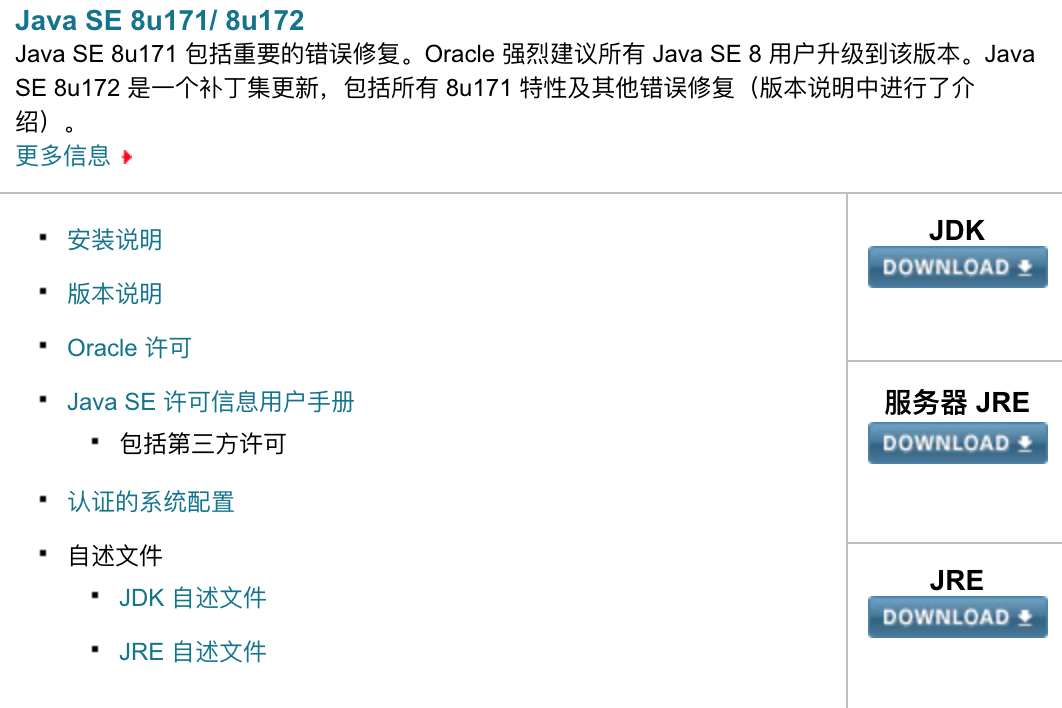
\includegraphics[height=150pt]{figures/oracle_jdk_download}
    \item 双击安装
  \end{enumerate}
\end{frame}

\begin{frame}
  \frametitle{认识JDK}
\end{frame}

\begin{frame}
  \frametitle{设置环境变量(可选)}
  环境变量一般是指在操作系统中用来指定操作系统运行环境的一些参数,这些参数一般以键值对的形式存在。
  
  Windows中可以通过“系统属性”->“高级”选项卡->“环境变量”对话框的方式增加、删除或者编辑修改环境变量。
  \begin{itemize}
    \item 增加\texttt{JAVA\_HOME}环境变量,将其赋值为JDK的安装目录:有些程序凭\texttt{JAVA\_HOME}寻找JDK的安装目录
    \item 修改\texttt{PATH}环境变量,将\texttt{JAVA\_HOME/bin}目录加入:使得可以在任何目录直接使用JDK提供的软件工具,如\texttt{javac}等
  \end{itemize}
  
  \begin{block}{\textbf{环境变量\texttt{PATH}的作用}}
    当你在计算机安装JDK之后,输入\texttt{javac}或者\texttt{java}之类的命令是不能马上被计算机正确执行的,因为计算机不知道到哪里去找这两个命令。那么计算机该如何查找你输入的命令呢? Windows操作系统是根据环境变量\texttt{PATH}来查找命令的。环境变量\texttt{PATH}的值是一系列路径,Windows操作系统将在这一系列的路径中依次查找命令对应的程序文件,如果能找到这个此命令,则该命令是可执行的;否则将出现“‘XXX’不是内部命令或外部命令,也不是可运行的程序或批处理文件”的提示。
  \end{block}
\end{frame}

\begin{frame}
  \frametitle{编写并运行第一个Java程序}
  \begin{enumerate}
    \item 使用任意纯文本编辑器(如记事本、np++等,不要使用Word)编写程序
    \item 使用\texttt{javac}编译程序
    \item 打开命令行窗口,使用\texttt{java}运行程序
  \end{enumerate}
  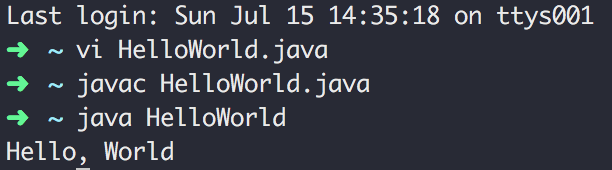
\includegraphics[width=\textwidth*2/3]{figures/hello_world}

\end{frame}

\begin{frame}[fragile]
  \frametitle{程序代码}
  \begin{enumerate}
    \item 右键新建“文本文件”,文件名为\texttt{HelloWorld.java}
    \item 使用记事本打开该文件,并逐行输入如下代码:
    \item 保存文件
  \end{enumerate}
\begin{javacode*}{label=HelloWorld.java}
public class HelloWorld {
   public static void main(String[] args) {
      // Prints "Hello, World"
      System.out.println("Hello, World");
   }
}
\end{javacode*}
\end{frame}

\begin{frame}
  \frametitle{Java源程序代码的基本组织形式}
  \begin{itemize}
    \item 源代码文件必须使用\texttt{.java}做为文件扩展名
    \item 源代码文件名(不包含扩展名)必须和代码中的类名相同!
    \item 源代码严格区分大小写
    \item 如果希望该源代码可以执行,必须定义程序入口函数,函数签名不能改变!\java|public static void main(String[] args)|
  \end{itemize}
  \begin{block}{\textbf{函数签名}}
    函数签名包含了:函数名、函数的参数列表、函数的返回值类型、函数的其他修饰
    \textbf{在Java中,函数也称为“方法”}
  \end{block}

\end{frame}

\begin{frame}
  \frametitle{编译和执行Java程序}
  \begin{enumerate}
    \item 打开命令行,使用\texttt{cd}命令切换到\texttt{HelloWorld.java}所在目录
    \item 编译Java源文件:\texttt{javac HelloWorld.java},得到字节码程序\texttt{HelloWorld}
    \item 执行编译后的字节码程序:\texttt{java HelloWorld},观察屏幕输出
  \end{enumerate}
\end{frame}

\begin{frame}
  \frametitle{代码风格(Code Style)}
  \begin{itemize}
    \item 代码风格又称编码风格、编码规范,是指编写源代码的书写风格,大体包括了:
      \begin{itemize}
        \item 如何给变量、函数、类命名
        \item 如何使用代码缩进
        \item 代码布局,如花括号的摆放位置等
      \end{itemize}
    \item 好的代码风格是出于工程上的要求,没有绝对的对错,只有好坏,代码风格的好坏和不同并不会直接导致程序出错
    \item 好的代码风格可以使得:
      \begin{itemize}
        \item 代码更美观、更加容易阅读理解
        \item 更容易发现编码过程中的错误
      \end{itemize}
    \item 很多人不重视代码风格,认为数学、算法才是根本,或者认为只要代码能运行,怎么书写并不重要。这种思想是错误的!因为正规的现代软件工程已经脱离了一个人小作坊式的编写模式,好的、统一的代码风格有助于提高团队工作效率!
  \end{itemize}
\end{frame}

\begin{frame}[fragile]
  \frametitle{本课程代码风格的要求(一)}
  本课程要求同学们编写代码时,必须遵守如下代码风格(这也是最常见的Java代码风格,参考Google编码风格制定):
  \begin{enumerate}
    \item 变量的命名采用\textbf{小驼峰命名法}:除第一个单词小写之外,其他单词首字母大写,如:\java|int studentCount|
    \item 类的命名采用\textbf{大驼峰命名法}:单词首字母均大写,如: \java|public class HelloWorld|
    \item 静态常量命名全大写,单词之间使用下划线(\texttt{\_})隔开,如: \java|public static final String CONSTANT_PI|
    \item 左花括号写在行末尾,不能新起一行;右花括号独占新的一行书写(也称K \& R 风格),如:
      \begin{javacode}
        public static void main(String[] args) {
        ... ...
        }  
      \end{javacode}
  \end{enumerate}
\end{frame}

\begin{frame}[fragile]
  \frametitle{本课程代码风格的要求(二)}
  \begin{enumerate}
    \setcounter{enumi}{4}
    \item 即使是可选的情况下,也要使用大括号,如:
      \begin{javacode}
        if (count > 6) { //此花括号在语法上可以省略,但是按照我们的代码风格,予以保留
          flag = true; 
        }  
      \end{javacode}
    \item 除非在for循环的定义中,操作符、运算符两边需各有一个空格(做为一个整体的操作符中间不需要加空格,如\texttt{!=}),如:\java|int studentCount = 10 - 1;|
    \item 如果字符的前面是逗号或分号,需要在前加一个空格:\java|for (int a=0; a++; a<10)|
    \item 小括号和中括号前留一个空格,后面不留空格

  \end{enumerate}
\end{frame}

\begin{frame}[fragile]
  \frametitle{本课程代码风格的要求(三)}
  \begin{enumerate}
    \setcounter{enumi}{8}
    \item 采用四个空格或者一个制表符tab做为一个缩进层级
    \item 一行最多只有一个以分号结尾的语句,一行最长100个字符
    \item 不要像C语言那样在函数头部一次性声明很多变量,用到的时候再声明
  \end{enumerate}
  
  \begin{javacode*}{label=错误代码风格举例}
    int a=3; //等号前后需要由空格
    double d = 1.0; double c = 2.0; //一行只应写一个带分号的语句
    public class studentScore {} //类名应该采取大驼峰写法,第一个单词首字母应大写
    static final String numCount; //静态常量应全部使用大写,单词间使用下划线隔开
    String student_name; //变量名应采取小驼峰写法
    
    public void getScore()
    {//此为C的代码风格,本课程中左花括号应写在函数声明行的最后
    return this.score; //此处应该有四个空格或者一个tab的缩进
    } 
  \end{javacode*}

\end{frame}

\begin{frame}[fragile]
  \frametitle{代码注释}
  \begin{columns}
  \column{0.5\textwidth}  
  注释的类型:
\begin{itemize}
  \item 单行注释:
\begin{javacode}
// 我是单行注释!
\end{javacode}
  \item 多行注释:
\begin{javacode}
/* 我是 
* 多行注释!
*/
\end{javacode}
  \item 文档(\texttt{javadoc})注释:
\begin{javacode}
/**
* 演示了文档注释
* @author Ayan Amhed
* @version 1.2
*/
\end{javacode}
\end{itemize}
\column{0.5\textwidth}
为什么必须写注释:
\begin{itemize}
  \item 你的代码可能是要被别人阅读的,别人可能不理解你的逻辑
  \item 你的代码自己以后也要重新阅读,你自己可能也不能理解写作代码当时的逻辑
  \item 写作代码时,帮助自己理清思路
\end{itemize}
\begin{block}{\textbf{注意}}
  注释是程序代码的有机组成部分,一边写代码,一遍写注释。本课程作业要求同学们必须写注释解释自己的思路!
\end{block}
  \end{columns}
\end{frame}

\begin{frame}
  \frametitle{集成开发环境(IDE)}
  \begin{itemize}
    \item IntelliJ IDEA:功能强大,高度集成,易于使用。除了Java也可作为常见绝大多数语言的开发环境
      \begin{itemize}
        \item 社区版(Community):免费使用
        \item 旗舰版(Ultimate):商业使用收费,教育和开源项目免费
      \end{itemize}
    \item Eclipse:功能强大,开源,免费。有多个版本,分别打包了不同的插件,用于Java SE、Java Web等开发
    \item NetBeans:功能强大,开源,免费,使用人数较前两者更少
  \end{itemize}
  
  \begin{block}{\textbf{IDE的选择}}
	\begin{itemize}
		\item 个人开发程序:三种IDE都很成熟,都可以很好的开发Java程序,写不好程序和IDE的选择无关!
		\item 团队开发程序:尽量和团队其他人使用的IDE保持一致
		\item 本课程选择IntelliJ IDEA进行授课,因为该IDE更加遵守Java项目的最佳实践,且大家以后如果学习Android,官方推荐的也是该IDE的衍生产物
	\end{itemize}
  \end{block}

\end{frame}
